\section{Docker}\label{DockerInstal}

Docker vereinfacht die Anwendungsbereitstellung, indem es den Transport und die Installation von Containern erleichtert, die alle erforderlichen Pakete als Dateien enthalten. Container gewährleisten die Trennung und Verwaltung der auf einem Computer verwendeten Ressourcen. Dazu gehören nach Angaben der Entwickler: Code, Laufzeitmodul, Systemwerkzeuge, Systembibliotheken - eben alles, was auf einem Computer installiert werden kann.
\begin{enumerate}
    \item Zunächst muss der Installations-Client für \href{https://docs.docker.com/docker-for-windows/install/}{Docker} heruntergeladen werden. Den Link dazu finden Sie hier:\href{https://docs.docker.com/docker-for-windows/install/}{https://docs.docker.com/docker-for-windows/install/}\\\\\textcolor{red}{Wichtig:} Für Windows wird entweder die Pro, Enterprise oder Education Version benötigt.
    
    \item Während der Installation von Docker werden Sie gefragt, ob Sie Windows Container oder Linux Container verwenden möchten. Stellen Sie sicher, dass Sie das Kästchen in der angezeigten Option nicht ankreuzen (vgl. Abbildung). Der Docker verwendet also Linux Contrainer. Docker-Container verwenden oft Linux-Komponenten, womit Windows-Container oft Probleme haben.\\
    \begin{center}
        \begin{minipage}[t]{0.5\textwidth}
            \centering
            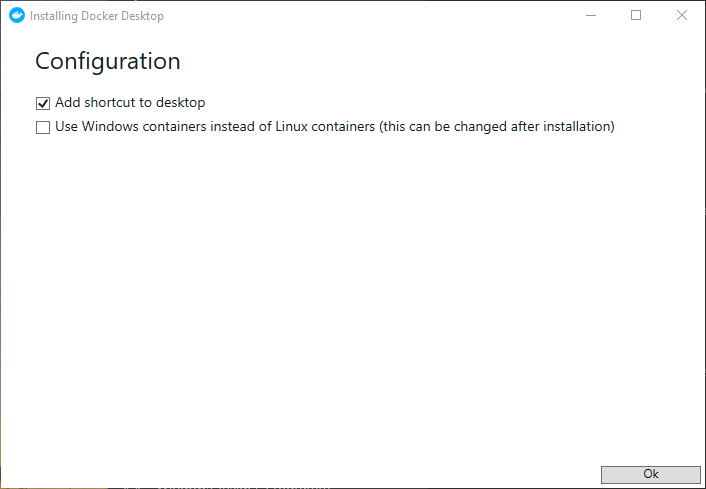
\includegraphics[width=(\textwidth)]{Kapitel3/DockerConfig.png}
            \captionof{figure}{Das Feld "Windows-Containers" sollte frei bleiben.}
            \label{ContainerConfig}
        \end{minipage}
    \end{center}

    \item Unter Windows müssen Sie Hyper-V und Container aktivieren. Hyper-V und Container können unter den Windows-Funktionen aktiviert werden. Dazu drücken Sie zunächst die Windows-Taste + Q und geben dort die Windows-Features ein. Aktivieren Sie dann Hyper-V und Container und klicken Sie auf "OK". Folgen Sie dann der Windows-Installation und installieren Sie die Features. Nach der Installation der Windows-Features müssen Sie den PC neu starten.\\\\\textcolor{red}{Wichtig:} Um Virtualisierungsdienste nutzten zu können, müssen diese gegebenenfalls im Bios-System aktiviert werden.
    \begin{center}
        \begin{minipage}[t]{0.35\textwidth}
            \centering
            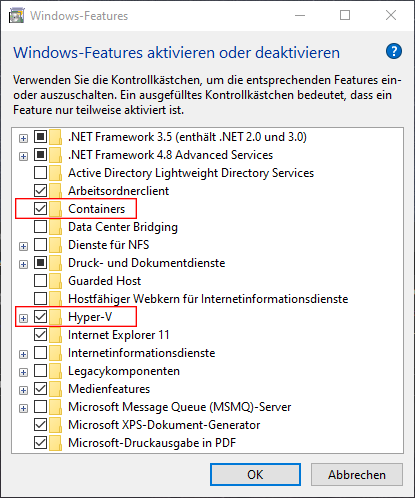
\includegraphics[width=(\textwidth)]{Kapitel3/WinFeature.png}
            \captionof{figure}{Benötigte Windows Features - Containers und Hyper-V.}
            \label{ContainerConfig}
        \end{minipage}
    \end{center}

    \item Es biete sich an unter Windows die "Windows PowerShell"{} zu nutzen, da diese für Docker nützliche Funktionalitäten im Gegensatz zur einfachen "Eingabeaufforderung"{} mit bringt. Wenn die Windows PowerShell noch nicht installiert wurde, können Sie es mit den Windows-Funktionen installieren. Drücken Sie dazu zunächst die Windows-Taste + Q und geben Sie "Windows-Feature" ein. Schalten Sie dann Windows PowerShell ein, und drücken Sie dann "OK". Installieren Sie PowerShell und starten Sie dann den Computer neu. 

    \begin{center}
        \begin{minipage}[t]{0.4\textwidth}
            \centering
            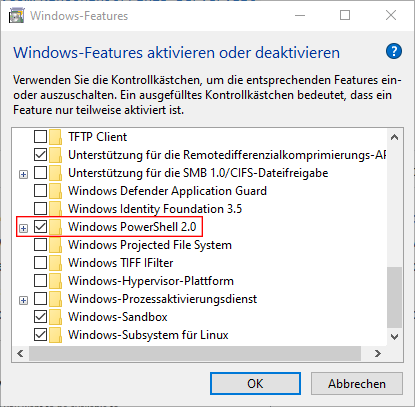
\includegraphics[width=(\textwidth)]{Kapitel3/WinPowerShell.png}
            \captionof{figure}{Benötigte Windows Features - PowerShell.}
            \label{ContainerConfig}
        \end{minipage}
    \end{center}


    \item Um nun einen Docker-Container unter Windows nutzen zu können, benötigt Docker noch Zugriff auf den Speicherort, auf welchem sich der Docker-Container befindet. Hierzu muss Docker Zugriff auf die Festplattenpartition gewährt werden, auf der die Docker-Container gespeichert sind. Um dies zu ermöglichen muss mit der linken Maustaste auf das Docker-Symbol in der Taskleiste das Einstellungsmenü geöffnet werden. Anschließen navigieren Sie zu dem Reiter "Resources / File Sharing"{}. Dort können Sie Docker Zugriff auf die Partitionen gewähren oder Sie wieder aufrufen. An diesem Punkt werden Sie auch nach dem aktuellen Windows-Benutzerkennwort gefragt. Sollten sie nach einem Passwort gefragt werden, geben Sie Ihr aktuelles Windows-Passwort ein, um Docker Zugriff auf die Partition zu gewähren. 
    
    \begin{center}
        \begin{minipage}[t]{0.8\textwidth}
            \centering
            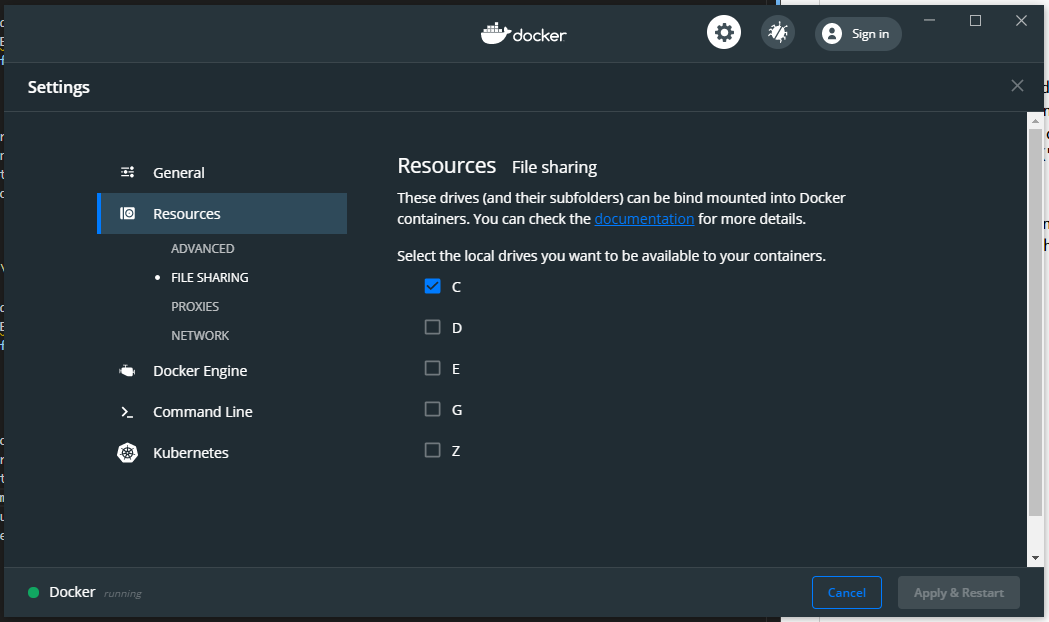
\includegraphics[width=(\textwidth)]{Kapitel3/DockerFiles.png}
            \captionof{figure}{Freigabe einzelner Partitionen für Docker.}
            \label{ContainerConfig}
        \end{minipage}
    \end{center}

\end{enumerate}
